\documentclass{article}
\usepackage[english]{babel}
\usepackage[utf8]{inputenc}
\usepackage{johd}
\usepackage{hyperref}
\usepackage{amsmath}
\usepackage{graphicx}
\usepackage{xcolor}

%%% title, author, date %%%
\title{%
  Philips Curve and Okun's Law in Mexico \\
    \vspace{3mm}
  \large Empirical Estimations on the Mathematical Model for the Macroeconomic Models}
\author{{Robin Mao, 1008267475, }\email{\href{mailto: robin.mao@mail.utoronto.ca}{robin.mao@mail.utoronto.ca}}}
\date{\small{March 27, 2023}}

%%% abstract %%%
\begin{document}
\maketitle
\begin{abstract}
    \noindent{This report will focusing on analyzing the Mexican Philips Curve and Okun's Law and give interpretations on the relations between the inflation rate, unemployment rate and output growth. It will analyze other economic factors and environments from a macroeconomic perspective. To ensure the mathematical accuracy, Python and its query-focused libraries such as Pandas, Geopandas and Numpy will be used, and the codes will be provided in a JupyterNotebook in Appendix.} \\
    \noindent{\textbf{Keywords: }{Philips Curve, Okun's Law, Inflation Rate, Unemployment Rate, Inflation Rate, Output Growth, Mexico}}
\end{abstract}

\vspace{3mm}
    
%%% introduction %%%
\section{Introduction}
    \hspace{5mm}{The major economic concepts of this essay are Philips Curve and Okun's Law. Philips Curve shows the relation between the inflation rate and the unemployment rate, and is often used by policymakers to understand economic conditions such as nominal wages and the inflationary environment. On the other hand, Okun's Law describes the relation between the change in unemployment rate and the change in real gross domestic product (referred latter to as GDP), which is another tool for authorities to examine the national economic development.}
    
    {This report will focus on the mathematical aspects of both concepts and provide interpretations and explanations. It will provide an estimated Philips Curve and an estimated Okun's Law equation for the current Mexican economy. We will begin by examining the economic factors (inflation rate, unemployment rate and real GDP) individually then plot the relations and create the estimators.}
    
%%% inflationary environment %%%
\section{Inflationary Environment in Mexico}
    \hspace{5mm}{The Mexcian inflation rate data set, provided by the World Bank $^{(1)}$, is calculated by the Consumer Price Index (referred latter to as CPI), which is a common inflation measurement that tracks the price of a goods basket and the services that are typically consumed by a household. It estimates the inflation rate by calculating the change in price over the change in time, which is an literal explanation of the following equation,}
        \begin{equation}
            CPI_t = \frac{C_t}{C_0} * 100
        \end{equation}
        
    {Where $C_t$ represents the basket price at time t, and $C_0$ represents the basket price in the base year. World Bank data set provides the Mexican inflation data from 1960 to 2021. The \textbf{CPI inflation rate} is calculated by finding the percent change in CPI over time. Here below are the statistics of the most recent 14 years. Note that the inflation is estimated calculating the CPI annually.}
    
    \begin{center}
        {Table: The Mexican Inflation Rate from 2008 to 2021} \\
        \vspace{1mm}
        \begin{tabular}{||c & c & c & c||}
            \hline
            2008 & 2009 & 2010 & 2011 & 2012 & 2013 & 2014 \\ [0.5ex]
            \hline
            5.124983 & 5.297356 & 4.156727 & 3.407378 & 4.111510 & 3.806391 & 4.018616	\\
            \hline \hline
            2015 & 2016 & 2017 & 2018 & 2019 & 2020 & 2021 \\ [0.5ex]
            \hline
            2.720641 & 2.821708 & 6.041457 & 4.899350 & 3.635961 & 3.396834 & 5.689208 \\
            \hline
        \end{tabular}
    \end{center}

    {Data above shows two major distribution nodes, one in 2008 and one in 2021. However, to ensure the precision, let us visualize the entire data set.}

\pagebreak

    {Using the World Bank data set and Matplotlib from Python, the data is visualized below.}
    \begin{center}
        \vspace{1mm}
        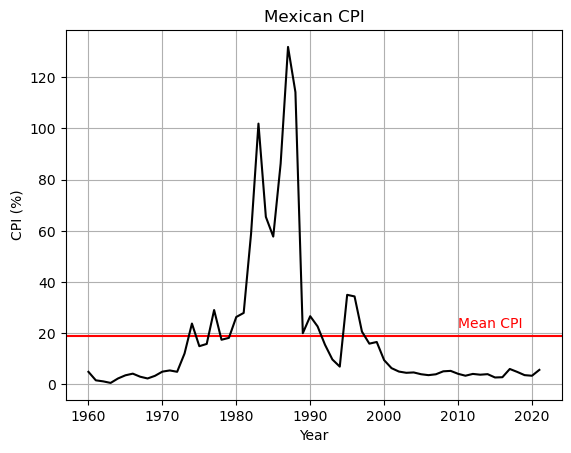
\includegraphics[width=9cm, height=7cm]{Mexican CPI Change Plot.png} \\
        \textcolor{gray}{\footnotesize{(Plot: the Mexican inflation rate estimated by CPI. Note that the graph is original.)}}
    \end{center}
    
    {The plot above demonstrates the variation in the Mexican Consumer Price Index. From the plot, we can see a major inflation node between 1980 and 1990, which was during the Mexican Financial Crisis$^{(2)}$. It was caused by an earthquake in Mexico City that caused more than 10,000 deaths and caused heavy economic damages. Furthermore, the ignorance from the governmental institutes on this tragedy had lead to another civic action, and another massive hurricane in 1988. There still exist fluctuations after the major events happened during the 80s and the 90s, however, they are relatively weak.}


%%% unemployment rate in Mexico %%%
\section{Changes in the Mexican Unemployment Rate}

    \hspace{5mm}{Mexico's unemployment rate has varied significantly over time, reflecting the country's economic and political changes. Historically, Mexico has experienced relatively high levels of unemployment, with peaks occurring during times of economic crisis and recession.}

    {Unemployment is the essential connection between the Philips Curve and Okun's Law, as former shows the relation between inflation and the unemployment and the latter shows the relation between the changes unemployment rate and the change in GDP.}

    {Unemployment rate is calculated by calculating the ratio between the unemployed population and the labour force, in which labour force is defined to be all the social members that are eligible to work and is actively seeking for jobs. Its mathematical calculation is given below,}

    \begin{equation}
        U = \frac{Unemployed Count}{Labour Force} * 100
    \end{equation}

    {In economic medium run (and long run), the national unemployment rate should remain at its \textbf{natural rate of unemployment}, which represents the unemployment rate of an economy when it is in its healthiest condition.}

    {World Bank provides the historical Mexican unemployment rate from 1991 to 2021$^{3}$. The detailed DataFrame is shown in the coding file in the end. The table below shows the most recent 14 years of the Mexican unemployment rate data.}

    \begin{center}
        {Table: The Mexican Unemployment Rate from 2008 to 2021} \\
        \vspace{1mm}
        \begin{tabular}{||c & c & c & c||}
            \hline
            2008 & 2009 & 2010 & 2011 & 2012 & 2013 & 2014 \\ [0.5ex]
            \hline
            3.870000 & 5.360000 & 5.300000 & 5.170000 & 4.890000 & 4.910000 & 4.810000	\\
            \hline \hline
            2015 & 2016 & 2017 & 2018 & 2019 & 2020 & 2021 \\ [0.5ex]
            \hline
            4.310000 & 3.860000	& 3.420000 & 3.270000 & 3.480000 & 4.450000 & 4.090000 \\
            \hline
        \end{tabular}
    \end{center}

    {The table above shows a node between 2009 to 2011, which is more than 1 percent higher than the rest. However, let us further plot the data to show the precise distribution.}
    
\pagebreak

    {Using the World Bank data set$^{(3)}$, we can plot the graph as below.}

\begin{center}
    \vspace{1mm}
    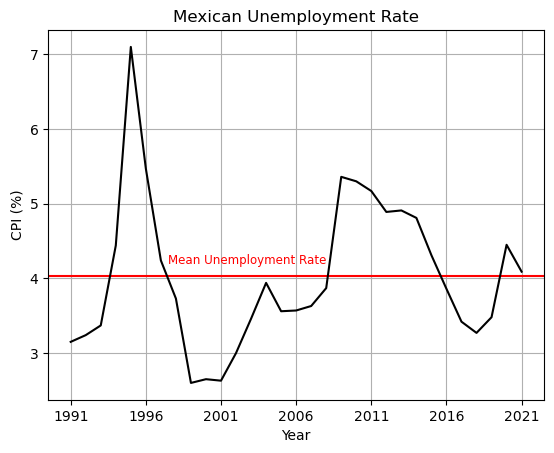
\includegraphics[width=9cm, height=7cm]{Mexican Unemployment Rate Change.png}
\end{center}

    {We can see several unemployment rate fluctuations in the graph. One is the historical peak around 1996 reaching 7 percent, which is resulted from the Mexican Peso Crisis when the overall household income decreased over 30 percent$^{(4)}$. Thus we can infer that the Mexican economy is in a recession around 1996.}

    {The unemployment rate dropped below the historical mean around 2001 when the economy was in its boom state. Then another recession hits around 2008 with a rising unemployment rate.}

    {The National Institute of Statistics and Geography $^(5)$ shows that the Mexican natural rate of unemployment is expected to be between 3 percent and 5 percent, in which our unemployment rate falls within the expected interval.}

    {Compare to the CPI graph in part two, where there exists a inflation node around 1995, we can see some relation between the two economic factors. However, we will first analyzed each factor individually, then make connections and correlations.}


%%% real GDP %%%
\section{The Mexican Real GDP Change}

    \hspace{5mm}{Gross Domestic Product (GDP), probably the most well-known macroeconomic statistic, is a measurement of the output of a nation. Compare to the nominal GDP, real GDP is adjusted to inflation to demonstrate a more accurate representation on the aggregate output of a country. One way to calculate this is the \textbf{Chain Weighting Method}:}

    \begin{equation}
        g_1 = \frac{\sum P_{t-1} * Y_t}{\sum P_{t-1} * Y_{t-1}}
    \end{equation}

    \begin{equation}
        g_2 = \frac{\sum P_t * Y_t}{\sum P_t * Y_{t-1}}
    \end{equation}

    \begin{equation}
        g_{t} = (\sqrt{g_1 * g_2} - 1) * 100
    \end{equation}

    {Where $g_1$ represents the growth rate using last year as the base year while $g_2$ represents it using this year as the base year. Then equation (5) calculates the geometric average and calculate the change.}

    {World Bank provides the Mexican Real GDP data set from 1960 to 2021, in USD billions. Thus the data is manually queried using the current exchange rate into the Mexican peso. Again, let us input the most current 14 years data into the table below.}

    \begin{center}
        {Table: The Mexican Real GDP from 2008 to 2021 (in trillion Mexican Peso)} \\
        \vspace{1mm}
        \begin{tabular}{||c & c & c & c||}
            \hline
            2008 & 2009 & 2010 & 2011 & 2012 & 2013 & 2014 \\ [0.5ex]
            \hline
            1.1099 & 0.9000 & 1.0578 & 1.1804 & 1.2010 & 1.2744 & 1.3153	\\
            \hline \hline
            2015 & 2016 & 2017 & 2018 & 2019 & 2020 & 2021 \\ [0.5ex]
            \hline
            1.1718 & 1.0784	& 1.1589 & 1.2224 & 1.2690 & 1.0905 & 1.2738 \\
            \hline
        \end{tabular}
    \end{center}

    {From table, we can see an increasing trend after the sudden drop in 2009, when the unemployment rate is relatively high (from graph above). Let us visualize the whole DataFrame.}

    \begin{center}
        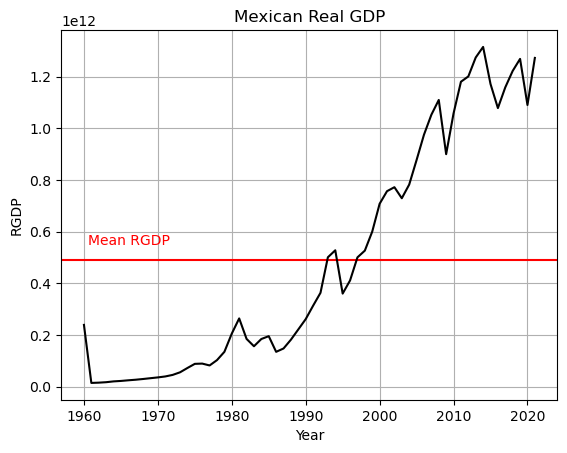
\includegraphics[width=9cm, height=7cm]{Mexican RGDP change.png} \\
        \textcolor{gray}{\footnotesize{(Note that the all graphs are original.)}}
    \end{center}

    {The graph above demonstrates the Mexican Real GDP changes in trillion Peso. It shows mainly an increasing trend with several fluctuations evenly distributed within. With the current DataFrames, we can now compare between the changes in the Inflation Rate, Unemployment Rate and Real GDP in the Mexican economy overtime. }

%%% comparsion %%%
\section{Comparison between the Factors}

    \hspace{5mm}{To ensure the statistical precision, the data sets are committed outer merges (all observations must have all three factors available to be remained in the DataFrame). After the merges, we have all available data from 1991 to 2021.}

    \begin{center}
        \small{Table: The Mexican RGDP, unemployment rate and inflation rate over time}\\
        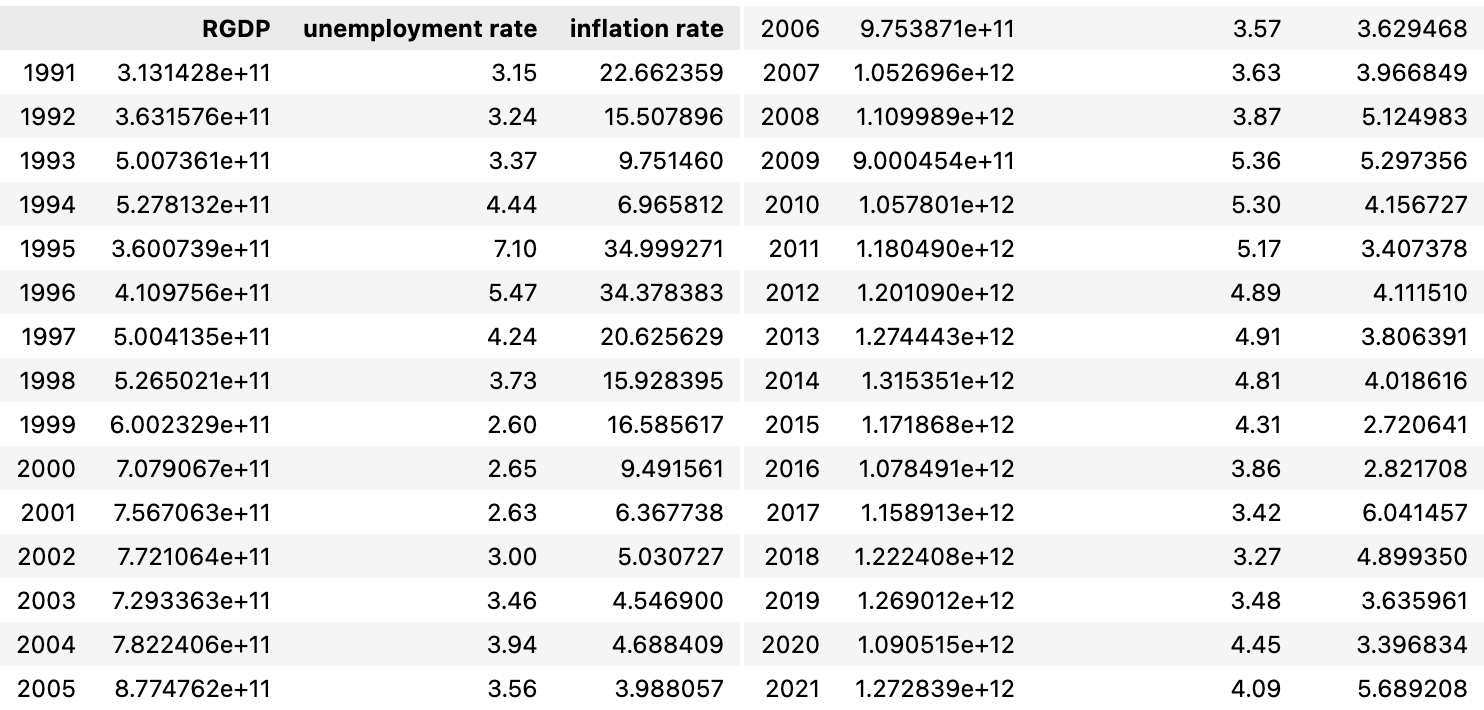
\includegraphics[width=14.84cm, height=7.10cm]{df_all_variable_table.png}\\
        \small{(Note that all data are provided in the Appendix Notebook.)}
    \end{center}
    
\pagebreak

    \begin{center}
        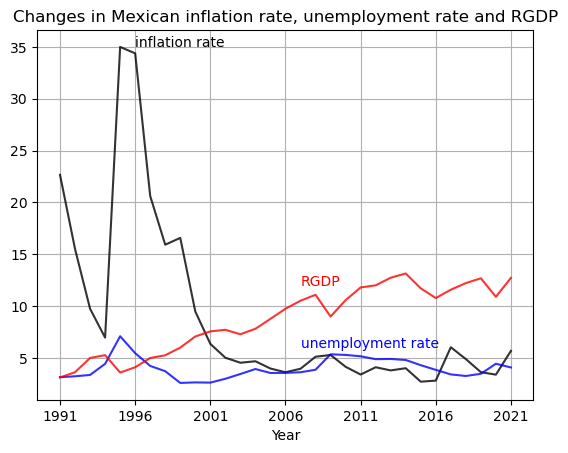
\includegraphics[weidth=9cm, height=7cm]{all_graphs.png}\\
        \textcolor{gray}{\footnotesize{Note that to analyze the trend, the RGDP has been simplified to its $\frac{1}{100,000,000}$ in Peso.}}
    \end{center}

    {The graph demonstrates a major inflation around 1996 with an decreased RGDP and increased unemployment rate. Most other minor fluctuations also follows the negative correlation between the unemployment rate and RGDP growth rate (as change in unemployment rate rises the RGDP growth rate decreases) and the positive correlation between the inflation rate and unemployment rate(the unemployment rate increases as the inflation rate rises). These trends are useful towards the estimation on the Philips Curve and Okun's Law in the upcoming section.}

%%% estimation on philips curve %%%%
\section{Estimation on the Philips Curve}

    \hspace{5mm}{Note that for this assignment, our target Philips Curve is modified into the following equation.}

    \begin{equation}
        \pi_t - \pi_{t-1} = \alpha(Y_t - \=Y)
    \end{equation}

    {Where $\pi_t$ is the inflation rate at time t, $Y_t$ is the RGDP at time t and $\=Y$ is the output gap. Note that if the output exceeds its output gap, the economy goes to a \textbf{boom}. The goal here is to estimate the coefficient $\alpha$.}

    \vspace{5mm}
    
    {To begin with, let us convert the Philips Curve into a more linear equation. }

    \begin{equation}
        \pi_t - \pi_{t-1} = a + b Y_t
    \end{equation}

    {Let us visualize the relation between the changes in Mexican inflation rate and the RGDP.}

    \begin{center}
        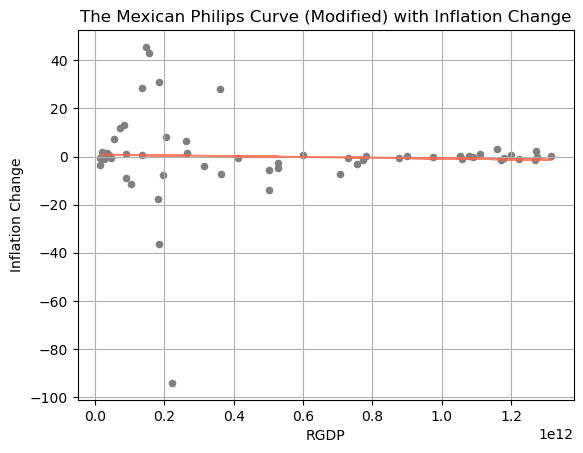
\includegraphics[width=9cm, height=7cm]{The Mexican Philips Curve.png}
    \end{center}

\pagebreak

    \begin{center}
        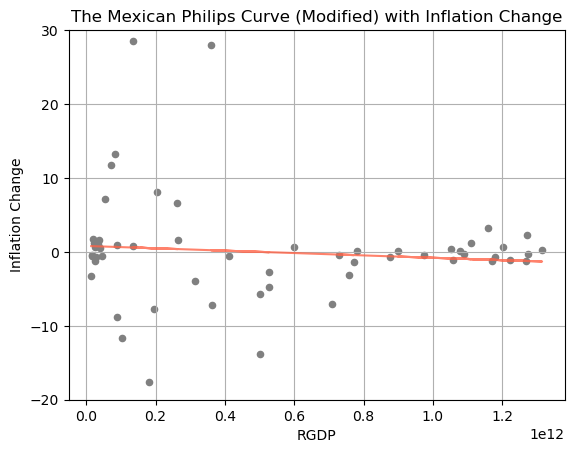
\includegraphics[width=9cm, height=7cm]{The Mexican Philips Curve Zoomed in.png}\\
        \textcolor{gray}{\footnotesize{\text{Plot: zoomed in}}}
    \end{center}
    
    {The scatter plot above demonstrates the Mexican Philips Curve with the unemployment rate modified to output with its linear regression. Note that the graph is original and obtained using DataFrames from above while linear regression is calculated using Numpy.polyfit.}

    {The coefficients from equation (7) are obtained as below.}

    \begin{equation}
        a = 0.804313644
    \end{equation}

    \begin{equation}
        b = -1.60257340 * 10^{-12}
    \end{equation}

    {Thus the linear equation is obtained as follow,}

    \begin{equation}
        \pi_t - \pi_{t-1} = 0.804313644 - 1.60257340 * 10^{-12} Y_t
    \end{equation}

    {Note that the unit of the output is Mexican Peso (individually) and all codes are provided in the JupyterNotebook in the Appendix. Different from the classic assumption, the computed $b$ coefficient is negative.}

    {Now let us manipulate the equation (10) into the equation (6) format.}

    \begin{equation}
        \pi_t - \pi_{t-1} = 0.804313644 - 1.60257340 * 10^{-12} Y_t = -1.60257340 (Y_t - 5.0189055 * 10^{11})
    \end{equation}

    {Where we can conclude that $\alpha$ = -1.60257340 and $\=Y$ = 5.0189055 * $10^{11}$ Peso.}
    
    {As $\alpha$ is negative and relatively large, it implies that for each $1*10^{11}$ Peso (demonstrated as $0.1*10^{12}$ in the graph above) increase in $Y_t$, the unemployment change decreases by 1.6025734\%.}

    {As the $\alpha$ coefficient is relatively small, the graph shows a significantly elastic relation between the RGDP and the inflation rate change. The size of $\=Y$ implies that the linear regression begins at a y-value of 5.0189055 * $10^{11}$ and is the estimated output gap of the Mexican economy. It is the national output when the economy is in its medium run or long run equilibrium, if exceeded, the economy goes to boom; vice versa, the economy experiences a recession. Overly, the sizes are expected due to the significant variation while the negative correlation is unusual.}

    {To examine the model accuracy, we calculate the coefficient of determination \textbf{$R^2$}, which represents the proportion of y-variation that can be explained by the model; error sum of squares \textbf{SSE}, total sum of squares which sums the total y-variation \textbf{SST} and the residual variance \textbf{$\sigma^{2}$}.}

    \begin{equation}
        SSE = \sum(e_i)^{2} = 18133.32493122715
    \end{equation}

    \begin{equation}
        SST = \sum{y_i - \=y} = 18165.025555294313
    \end{equation}

    \begin{equation}
        R^2 = 1 - \frac{SSE}{SST} = 1 - \frac{18133.32493122715}{18165.025555294313} = 0.001745146130990305
    \end{equation}

\pagebreak

    \begin{equation}
        \sigma^2 = \frac{SSE}{n-2} = \frac{18133.32493122715}{61-2} = 297.2676218233959
    \end{equation}

    {Where n is the number of observations. Thus we can conclude that the linear regression explains 0.1745146130990305 of the y-variation. This is due to the huge variance in the Mexican inflation change. However, utilizing \textbf{polynomial regression} and machine learning techniques, we can conclude a more accurate version as below,}

    \begin{equation}
        \pi_t - \pi_{t-1} = 2.67317472 - 1.59850531*10^{-11}Y_t + 1.17305673 * 10^{-23}Y_t^{2}
    \end{equation}

    {This polynomial regression provides a more accurate estimation on the two variables.}

    \begin{center}
        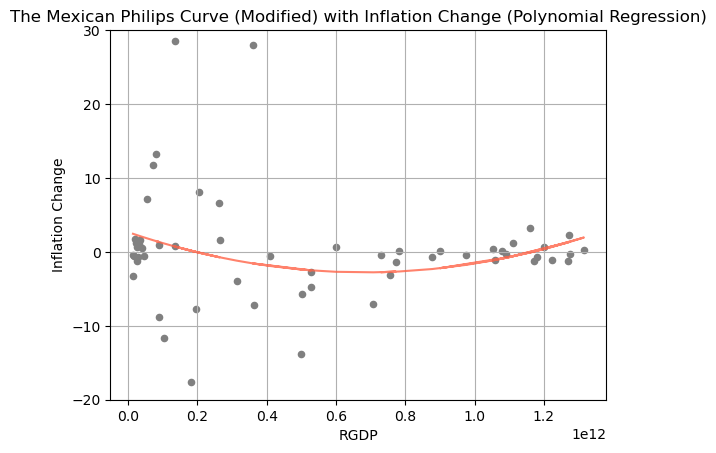
\includegraphics[width=10cm, height=7cm]{Philips Curve Polynominal.png}
    \end{center}

    {The $R^2$ of this model is 0.010034378706649805, which is almost 10 times higher than the linear regression model. Note that detailed calculations are included in the Notebook in Appendix.}

%%% estimation on the mexican okun's law %%%
\section{Estimation on the Mexican Okun's Law}

    \hspace{5mm}{Okun's Law is an macroeconomic concept that shows the (mostly negative) relation between the change in unemployment rate and the Real GDP growth. The mathematical relation is provided as below,}
    
    \begin{equation}
         u_t - u_{t-1} = - \beta (g_{yt} - g)
    \end{equation}

    {Where $u_t$ stands for the unemployment rate at time t, and $g_{yt}$ stands for the output growth at time t. The goal of this section is to provide an accurate estimation on the coefficient $\beta$.}

    \vspace{5mm}
    
    {Again, let us manipulate the equation (11) into a more linear form as below,}

    \begin{equation}
        u_t - u_{t-1} = a + b g_{yt}
    \end{equation}

    {With the World Bank DataFrames obtained in the previous sections, we can create the visualization of the Mexican Okun's Law as below,}

    \begin{center}
        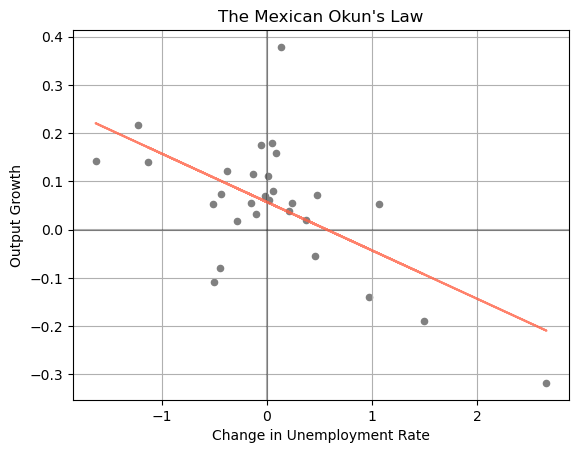
\includegraphics[width=9cm, height=7cm]{Mexican Okun's Law.png}
    \end{center}

    {The graph above demonstrates the negative relation between the Mexican output growth and the unemployment rate. Several outliners in the output growth rate are recorded. Note that different from the Philips Curve, Okun's Law uses the RGDP percent change as the y-vairable.}

    {The coefficient are calculated using Python and Numpy libraries mainly calling numpy.polyfit(). The coefficients are concluded as below,}

    \begin{equation}
        a = 0.05724077
    \end{equation}

    \begin{equation}
        b = -0.10027533
    \end{equation}

    {Thus equation (18) becomes}

    \begin{equation}
        u_t - u_{t-1} = 0.05724077 - 0.10027533*g_{yt}
    \end{equation}

    {Note that all codes and calculations are provided in the Appendix. This equation implies that for each one percent increase in the RGDP growth, the unemployment rate will decrease by 0.10027533 unit with the initial value of 0.05724077. With the DataFrames provided by World Bank, this is as much as we could estimate.}

    {Now let us manipulate the equation (21) into the Okun's Law format,}

    \begin{equation}
        u_t - u_{t-1} = 0.05724077 - 0.10027533*g_{yt} = - 0.10027533 * (g_{yt} - 0.57083602)
    \end{equation}

    {Which concludes that $\beta$ = 0.10027533 and g = 0.57083602\%. Note that both their signs are positive. Compare to other countries, the Mexican $\beta$ coefficient is relatively small, which implies a more elastic relation between the unemployment rate and the RGDP growth rate while g being relatively large. This is consistent with the classic assumption and the initial expectation because as the RGDP growth rate increases, labour demand rises, resulting in a lower unemployment rate.}

    {To examine the model accuracy, the variable $R^2$, which represents the proportion of y-variation that can be explained by the regression model, is calculated in the Notebook in Appendix. The calculation method is identical to section 6. The computed $R^{2}$ for the Mexican Okun's Law is given as,}

    \begin{equation}
        R^{2} = 0.37746473436939865
    \end{equation}

    {With the total sum of squares SST = 0.4971973087547591 and error sum of squares SSE = 0.30952285867646406. The estimated residual variance is given as, }

    \begin{equation}
        \sigma^2 = \frac{SSE}{n - 2} = \frac{0.30952285867646406}{29 - 2} = 0.011463809580609781
    \end{equation}

    {Thus we can conclude that the linear regression model can explain 37.746473436939865\% of the y-variation.}

\pagebreak

%%% conclusion %%%
\section{Conclusion}

    \hspace{5mm}{This report provides the mathematical estimations of the Mexican Philips Curve and the Mexican Okun's Law as below,}

    \vspace{5mm}
    
    {\textbf{Philips Curve}(with unemployment rate changed to output):}

    \begin{equation}
        \pi_t - \pi_{t-1} = -1.60257340 (Y_t - 5.0189055 * 10^{11})
    \end{equation}

    {With $R^2$ = 0.001745146130990305, SSE = 18133.32493122715, SST = 18165.025555294313 and $\sigma^2$ = 297.2676218233959. There is also a more precise polynomial estimation in equation (16).}

    \vspace{5mm}

    \textbf{Okun's Law:}

    \begin{equation}
        u_t - u_{t-1} = - 0.10027533 * (g_{yt} - 0.57083602)
    \end{equation}

    {With $R^2$ = 0.37746473436939865, SSE = 0.30952285867646406, SST = 0.4971973087547591, $\sigma^2$ = 0.011463809580609781.}

    \vspace{5mm}
    
    {The results indicates that there exists huge fluctuations in all the Mexican's Inflation Rate, Unemployment Rate and Real Gross Domestic Product with correlations countering some classic assumptions.}
    
%%% references %%%
\section*{References}
    
    \begin{enumerate}
        \item{Inflation, consumer prices (annual \%) - Mexico | Data. (n.d.). Data.worldbank.org. \\ https://data.worldbank.org/indicator/FP.CPI.TOTL.ZG?locations=MX}
        
        \item{History.com Editors. (2020, September 14). Hispanic History Milestones: Timeline. HISTORY. https://www.history.com/topics/hispanic-history/hispanic-latinx-milestones}
        
        \item{World Bank. (2021). Unemployment, total (\% of total labor force) (modeled ILO estimate) | Data. Worldbank.org. https://data.worldbank.org/indicator/sl.uem.totl.zs}
        
        \item{What Happened in 1996 - Significant Events, Prices, 25 years ago Top Movies, TV and Music. (n.d.). Www.thepeoplehistory.com. https://www.thepeoplehistory.com/1996.html}
        
        \item{CEICdata.com. (2018). Mexico Unemployment Rate. Ceicdata.com; CEICdata.com. \\
        https://www.ceicdata.com/en/indicator/mexico/unemployment-rate}
    \end{enumerate}


%%% appendix %%%
\section*{Appendix}

    {Disclaimer: all graphs are original. All calculations, DataFrames and codes are in the Notebook below.}

    \begin{itemize}
        \item{\textbf{JupyterNotebook: }\href{https://github.com/robinasaki/Philips-Curve-and-Okun-s-Law-in-Mexico.git}{https://github.com/robinasaki/Philips-Curve-and-Okun-s-Law-in-Mexico.git}}
    \end{itemize}

%%% end %%%
\end{document}